\subsubsection{Model architecture}
\label{sub:comb_model_architecture}

\structure{General architecture ideas \& requirements}
\outline{Basic idea: sequences (content features) are processed before merging 
with structured features (mainly contextual), combination via FC layer}
\outline{Text processing with convolutional and recurrent layers, as is common
practice in many NLP models}
\outline{Differences: RNNs take longer to train (limited parallelization 
possibilities, often magnitude of 3!), CNNs are feature detectors (e.g., sentiment, requests, specific terms), 
RNNs model features across time}
\outline{LSTM cells are used for RNNs, most widely adopted RNN cell type}
\outline{Input sequences have length 32, word embedding is 100-dimensional}
\outline{Since data sets are rather small for such a complex NLP task, models
are kept simple (avoids overfitting too quickly)}

\begin{figure}[h]
\begin{subfigure}{.5\textwidth}
  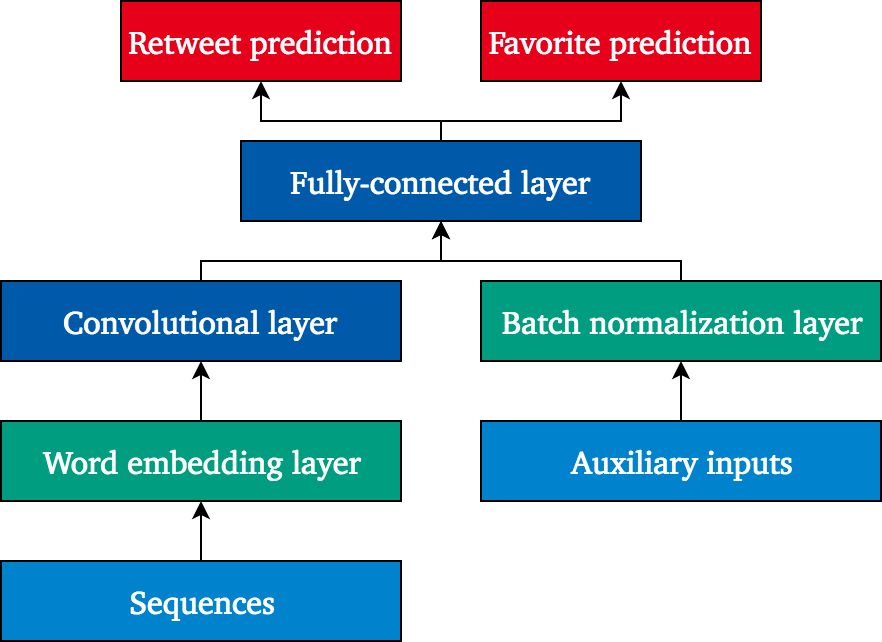
\includegraphics[width=.95\linewidth]{img/dm2_cnn}
  \caption{DM2-CNN}
  \label{fig:dm2_cnn}
\end{subfigure}%
\begin{subfigure}{.5\textwidth}
  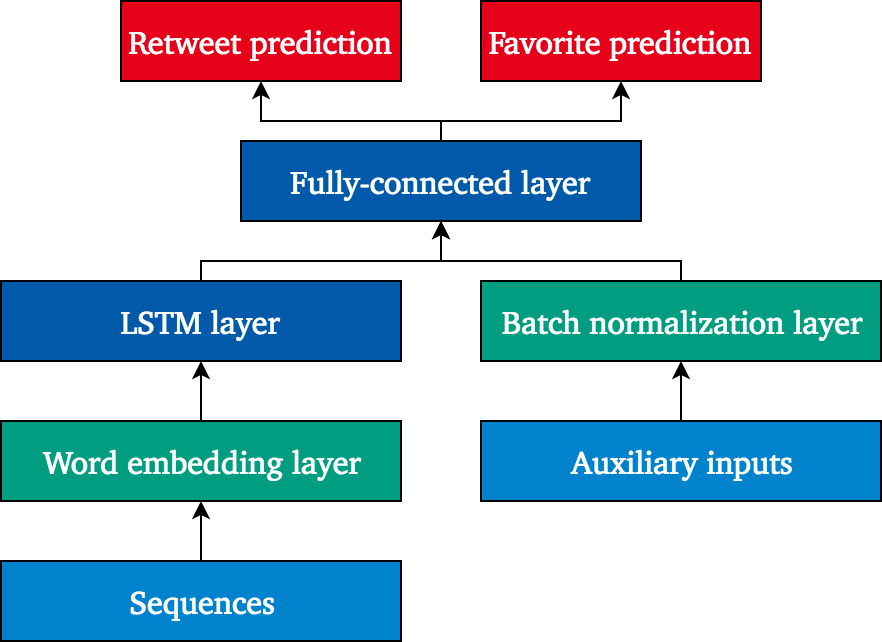
\includegraphics[width=.95\linewidth]{img/dm2_lstm}
  \caption{DM2-LSTM}
  \label{fig:dm2_lstm}
\end{subfigure}
\begin{subfigure}{.7\textwidth}
  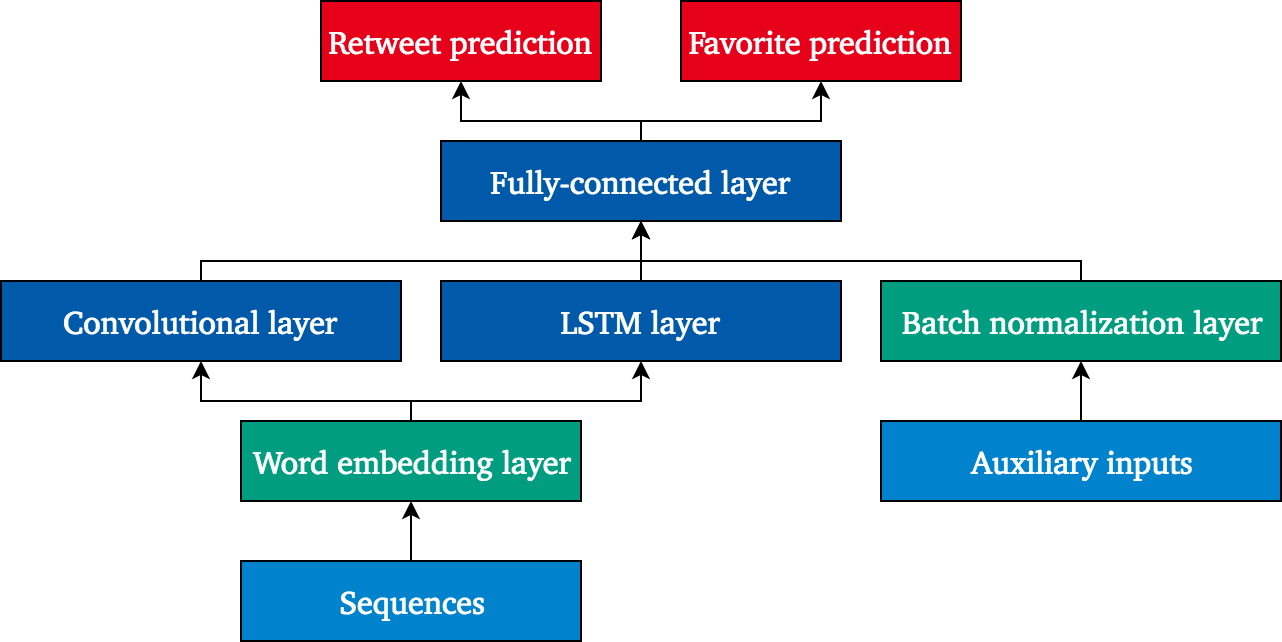
\includegraphics[width=.95\linewidth]{img/dm2_cnn_lstm}
  \caption{DM2-CNN-LSTM}
  \label{fig:dm2_cnn_lstm}
\end{subfigure}
\caption{Subset of evaluated architectures for multi-input models}
\label{fig:dm2_architectures}
\end{figure}

\structure{Model selection process}
\outline{Figure shows subset of tested architectures}
\outline{DM2-CNN applies single convolutional layer to sequences}
\outline{32 filters with size 3, padding before (keep sequence length) and max-pooling after conv layers}
\outline{DM2-CNN2 \& DM2-CNN3: same concept, but consecutive conv layers, enables
detection of more complex features, max-pooling after each layer (sequence
gets halved everytime)}
\outline{DM2-LSTM returns sequences, i.e., learned representation after each
input of the sequence (16-dimensional)}
\outline{DM2-CNN-LSTM combines both architectures, i.e., more features to combine}
\outline{Use of regularization: partly dropout after convolutions, batch
normalization after FC layer and for normalizing aux inputs}

\begin{table}
\begin{tabular}{llrr}
\toprule
Model architecture & Data set & Classification loss & Regression loss \\
\midrule
DM2-CNN & Combined & 0.7897 & \textbf{401.5174} \\
DM2-LSTM & Combined & 0.7628 & 411.2176 \\
DM2-CNN-LSTM & Combined & \textbf{0.7556} & 410.8704 \\
DM2-CNN2 & Combined & 0.7641 & 409.1842 \\
DM2-CNN3 & Combined & 0.8050 & 404.9901 \\
\bottomrule
\end{tabular}
\caption{Summary of multi-input model selection}
\label{tab:dm2_selection_results}
\end{table}

\structure{Selection results}
\outline{Selection was done on combined data set, since least prone to overfitting}
\outline{Architectures show similar performance, differences are not that big}
\outline{DM2-CNN chosen for regression: no regularization, 64 FC units}
\outline{DM2-CNN-LSTM chosen for classification: regularized via dropout after
conv layer, 128 FC neurons (intuitive since more features need to be combined)}
